\section{Numerical implementation} \label{sec:numerical_implementation}

As discussed in \sec{sec:radial_locality}, the radial kernels decay ($\propto ~ \beta^{-1.5}$) as the distance from the central pixel increases, but they begin to increase on approaching the diametrically opposite position ($\beta \rightarrow \pi$)  as seen in \fig{fig:rad_ker_decay}). For a sufficiently high maximum multipole $\ell_{\rm max}$, the lowest multipole being fixed at $\ell_{\rm min}=2$, the maximum the radial kernel reaches near the vicity of the diametrically opposite end can be significantly smaller than global maxima of the radial kernel. This suggests that for sufficiently high resolution CMB maps (${\rm NSIDE} >32$), having high multipole information, it may suffice to restrict the convolution over the Stoke parameters Q \& U (to deduce either the scalar E \& B maps or pure Stokes Q \& U corresponding to either of the two scalar modes) to a local region around the central pixel. The locality of the region is quantified by the non-locality parameter $\beta_o$, which is a function of the maximum multipole accessible in the Stokes maps.

We have developed a Python script to evaluate these local convolution over Stokes Q \& U parameters. To evaluate the convolution kernel (\eq{eq:qu2eb_convolution}), we precompute the radial part of the kernel ( $f(\beta), {}_{+2}f(\beta) ~\&~ {}_{-2}f(\beta))$. Specifically, we use the python routine {\textit scipy.special.lpmn} to evaluate the associated Legendre polynomial functions, which are needed to evaluate the radial kernels. $f(\beta)$ is simply evaluated by calculating the multipole sum in \eq{eq:rad_ker_queb}. ${}_{+2}f(\beta) ~\&~ {}_{-2}f(\beta))$ are estimated by evaluating the sum in \eq{eq:f2_rad_ker}, where we take care to use the limiting forms of the functions ${}_{\pm 2}f_{\ell}(\beta)$ in the vicinity of $\beta=0,\pi$ as discussed in \app{sec:asymptotic_f}. As the next step, for each pixel on the Healpix map we get the pixel numbers of all the neighboring pixels lying within radius of $r_{\rm cutoff}$ from the central pixel using the Healpix routine {\textit query\_disc}. We then use the {\textit pix2ang} function of Healpix to get the angular coordinates of the central $(\theta_o,\phi_o)$ and its surrounding pixels $(\theta_i,\phi_i)$, which are then used to calculate the corresponding Euler angles using \eq{eq:fn_euler}. Given these  inputs we evaluate the convolution kernel as simple Reimann sums. We repeat this procedure for each pixel on the Healpix map. 

For the results presented in the following sub-sections we work with CMB maps at Healpix resolution of ${\rm NSIDE}=64$, unless specified otherwise. \revisit{We use the CMB spectra for some fiducial cosmology. This work  only deals with lensing B-mode spectra.} To understand the effects of restricting the convolution to a local neighbourhood, we evaluate these convolutions on discs with progressively smaller radii surrounding the central pixel.  Specifically the non-locality parameter for a NSIDE=64 map is $\beta_o=30^{\circ}$. We impose radial cutoffs of $r_{\rm cutoff}=[2\beta_0,\beta_o,0.5\beta_o,0.25\beta_o]$ with an apodization of 3 degrees having a cosine squared profiles on the edges of the discs. We also evaluate the corresponding maps using standard Healpix routines and use these as reference maps for this exercise. Note that the Healpix evaluations are in principle equivalent to carrying out the convolution over the full sphere (i.e. $\beta_o=\pi$).  We compare the spectra derived from all these maps to those derived from the reference maps to quantify the effect of the imposed radial cutoff on the convolution integrals.

%--------------------------------------------------------
%--------------------------------------------------------
\subsection{Constructing E \& B maps from local convolutions on Stokes Q \& U maps}

%
\begin{figure}[!h] 
\centering
\subfigure[E-mode Healpix]{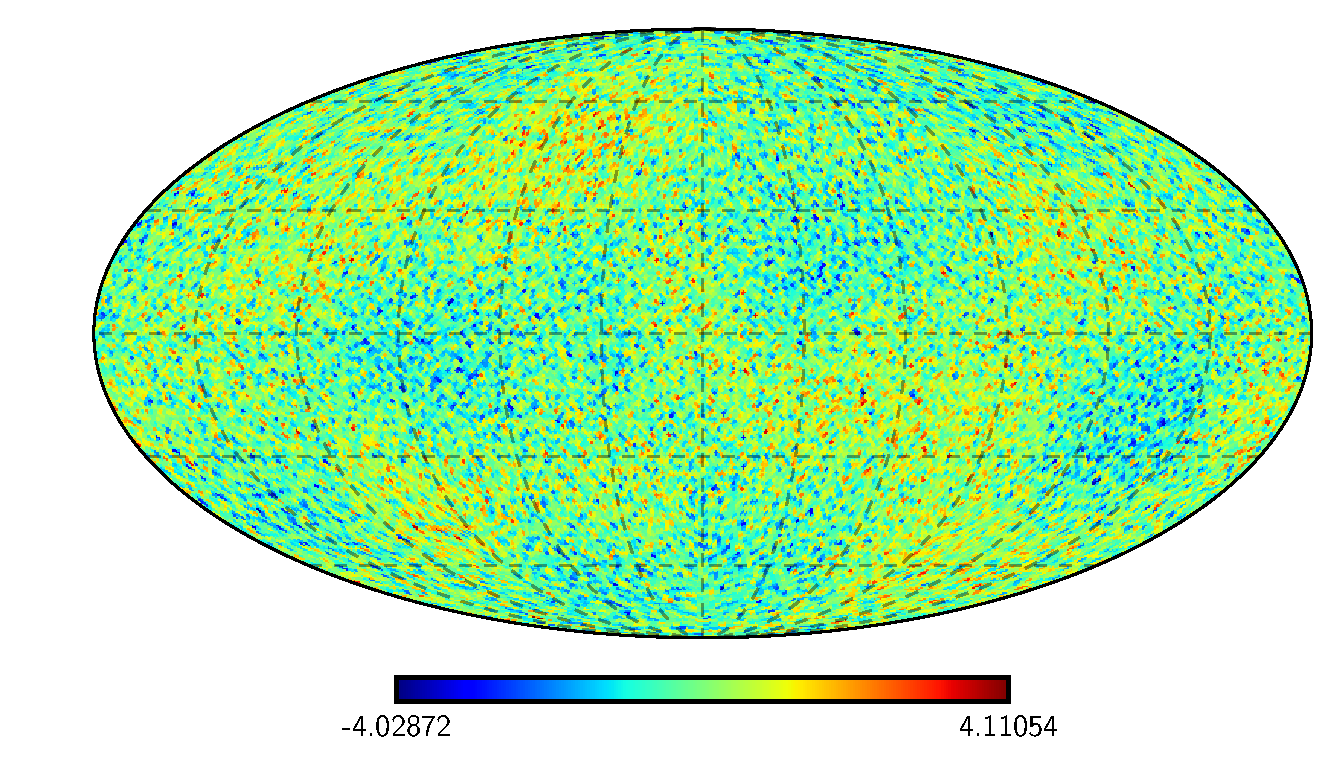
\includegraphics[width=0.31\columnwidth]{emap-healpix.pdf}}
\subfigure[E-mode local convolution]{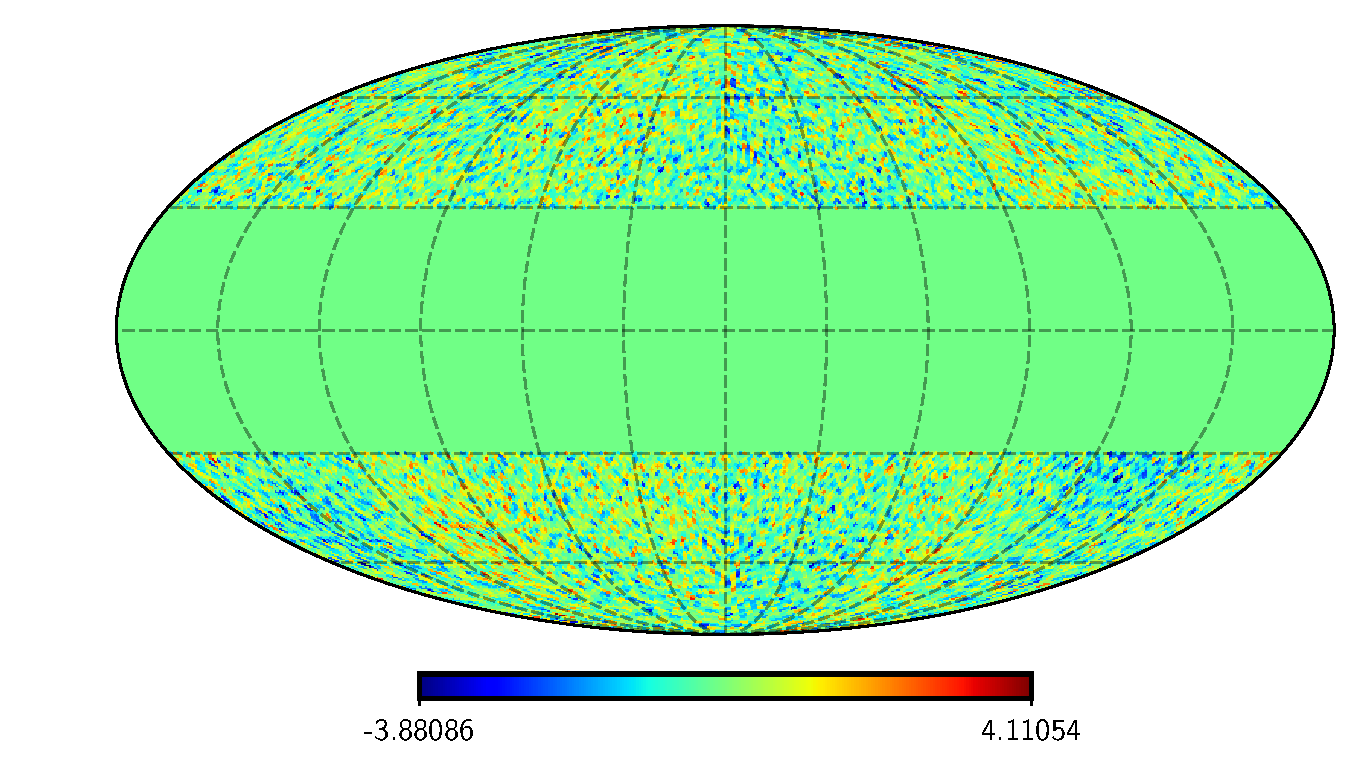
\includegraphics[width=0.31\columnwidth]{emap-2beta.pdf}}
\subfigure[Difference]{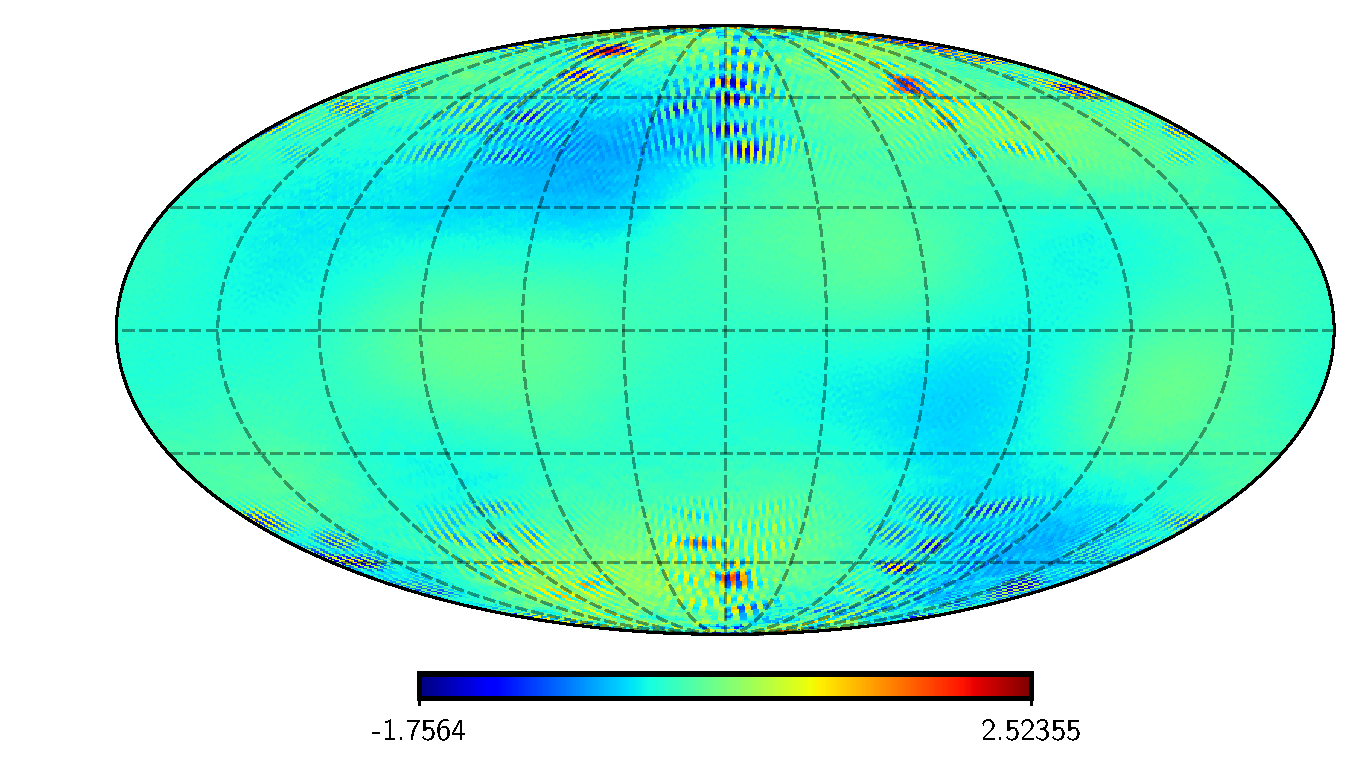
\includegraphics[width=0.31\columnwidth]{emap-diff.pdf}}
\subfigure[B-mode Healpix]{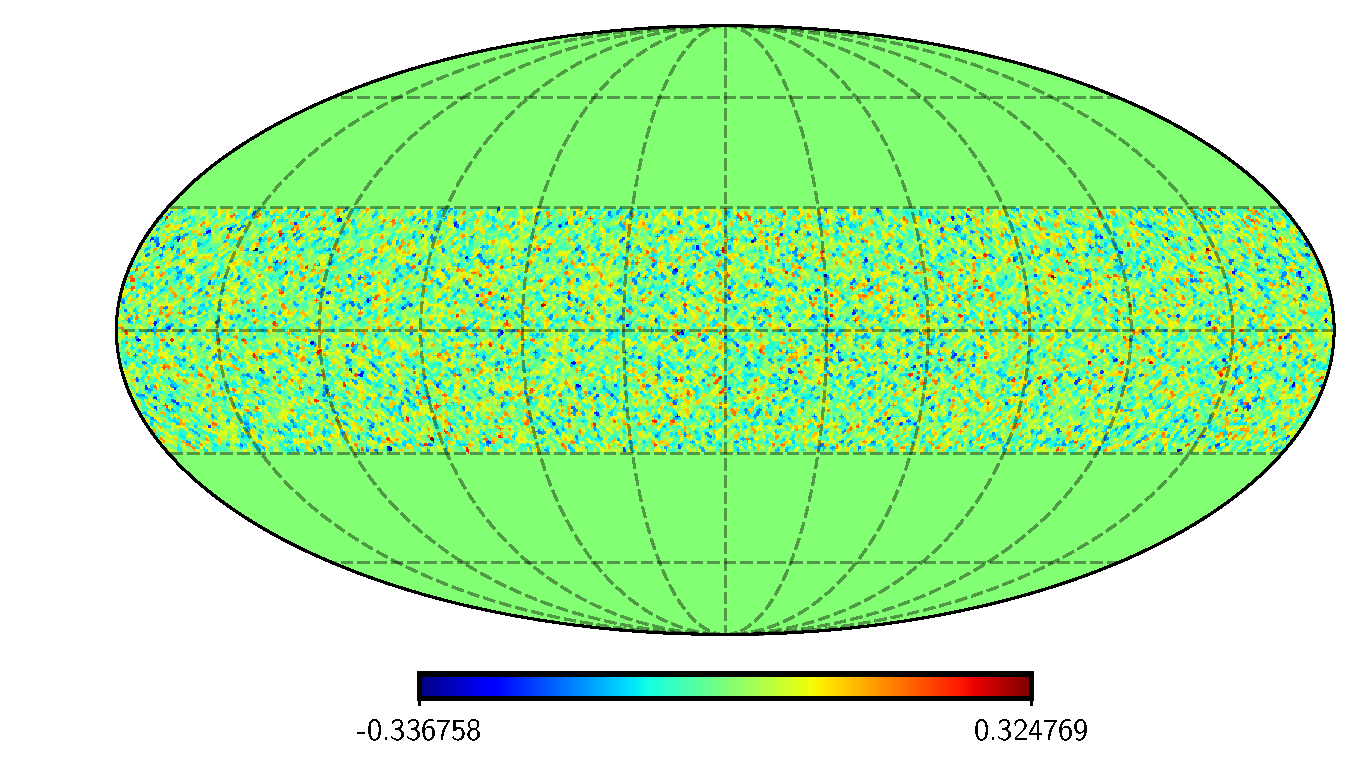
\includegraphics[width=0.31\columnwidth]{bmap-healpix.pdf}}
\subfigure[B-mode local convolution]{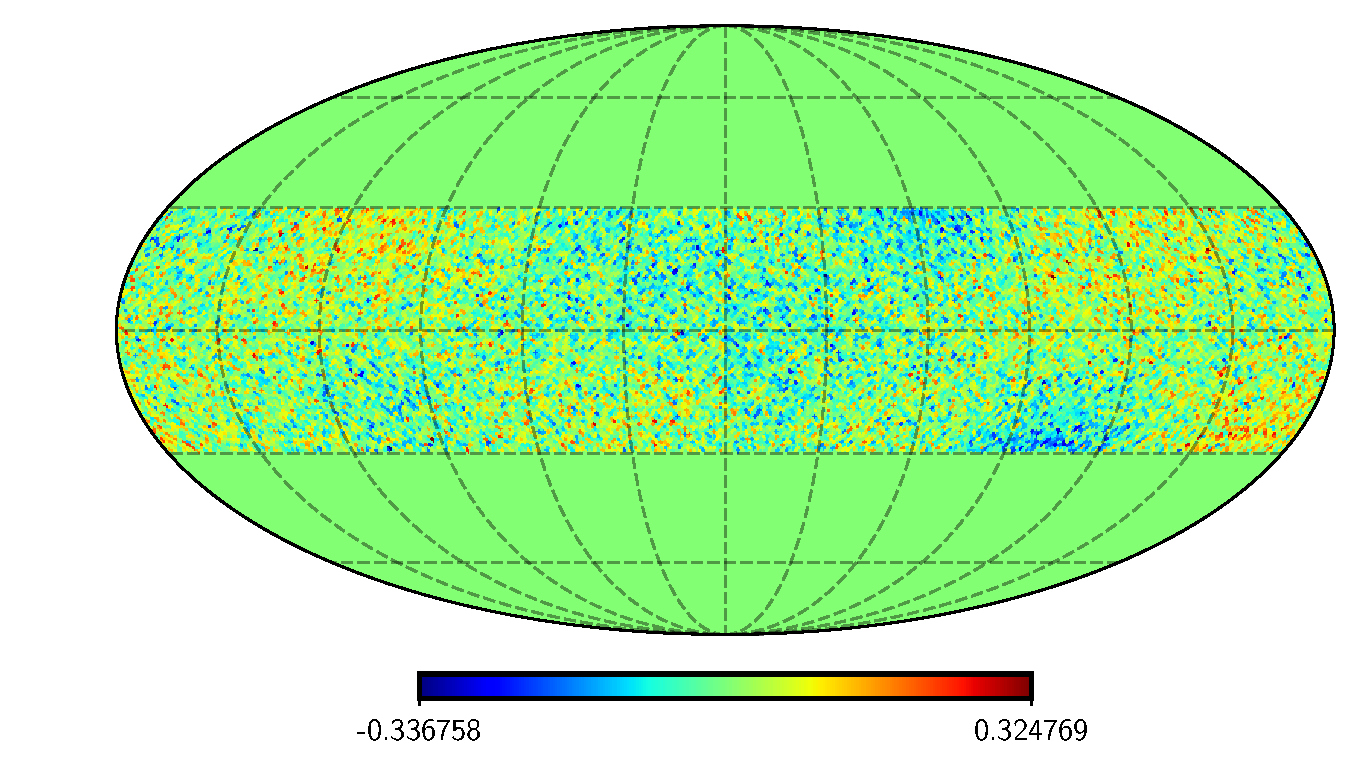
\includegraphics[width=0.31\columnwidth]{bmap-2beta.pdf}}
\subfigure[Difference]{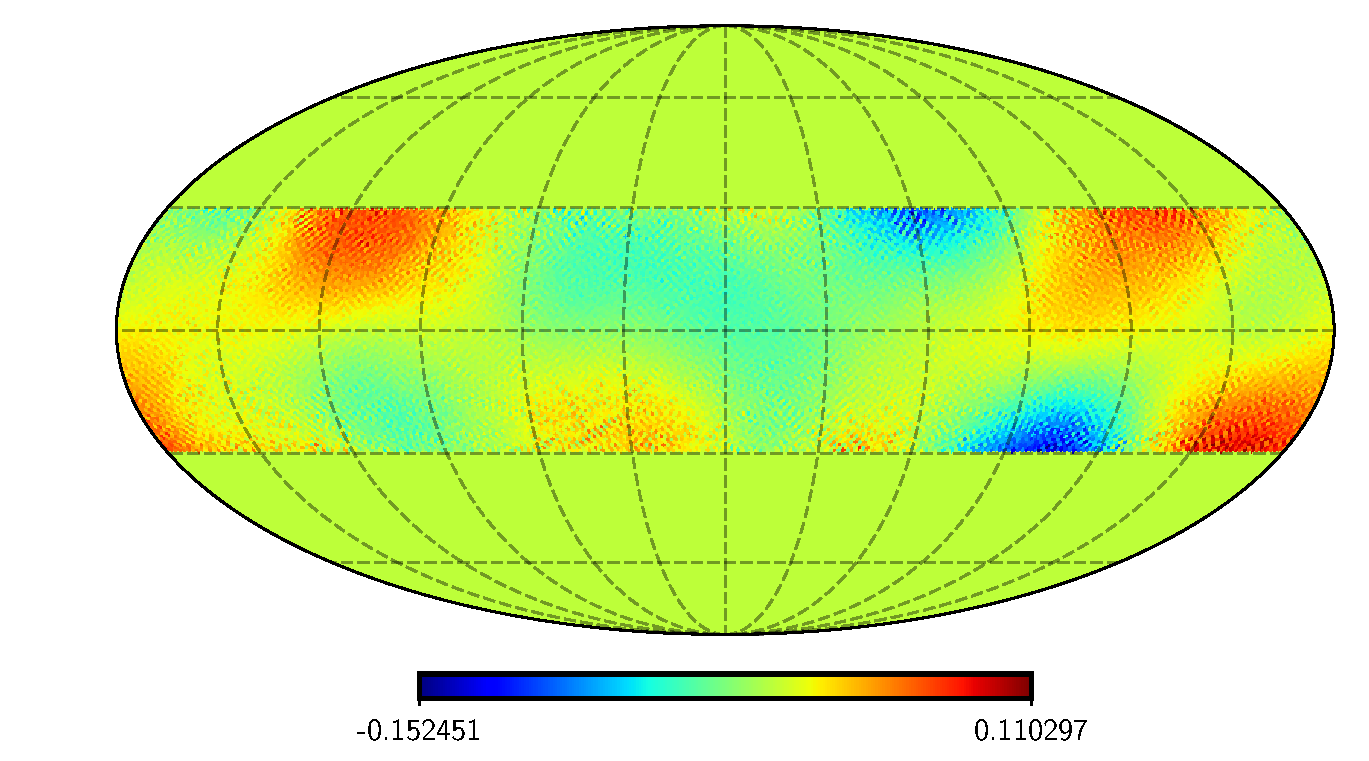
\includegraphics[width=0.31\columnwidth]{bmap-diff.pdf}}
\caption{{\textit Left:} Reference E \& B mode maps derived using Healpix. {\textit Middle:} E \& B mode maps derived using $r_{\rm cutoff}=2\beta_o$. {\textit Right:} Difference between the maps shown in the left and middle columns. Note that the differences maps are primarily due to differences in the recovery of large scale modes.}
\label{fig:eb-maps-compare}
\end{figure}
%
%
\begin{figure}[!h] 
\centering
\subfigure[]{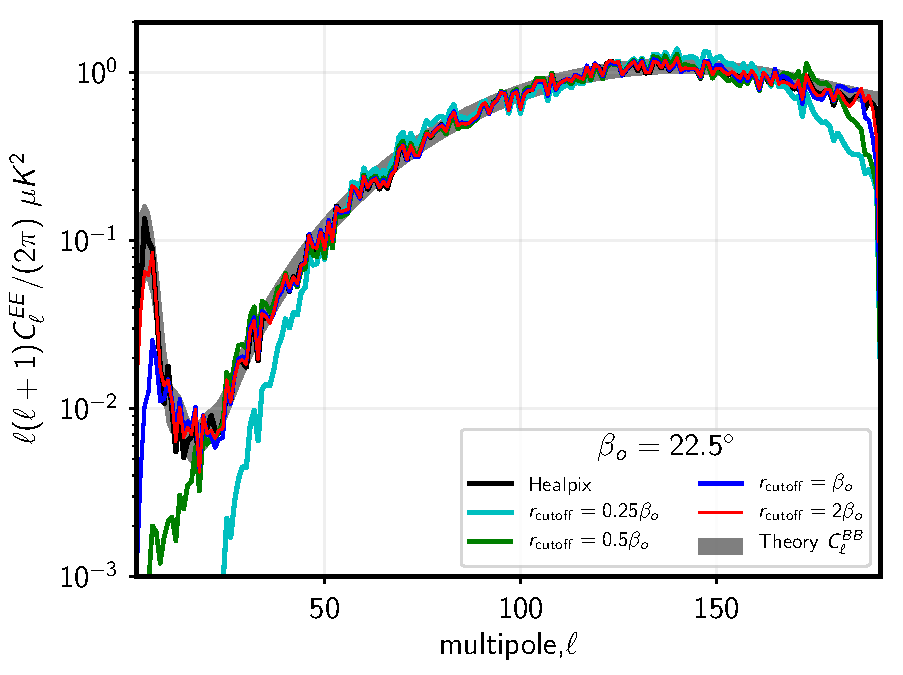
\includegraphics[width=0.49\columnwidth]{ee-spectrum-radial-cutoff.pdf}}
\subfigure[]{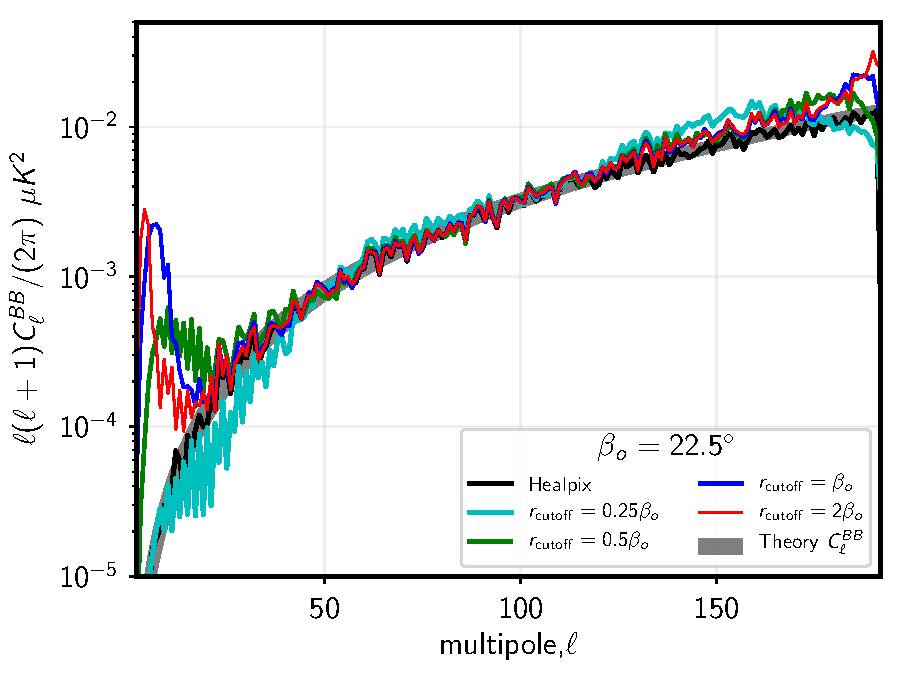
\includegraphics[width=0.49\columnwidth]{bb-spectrum-radial-cutoff.pdf}}
\subfigure[]{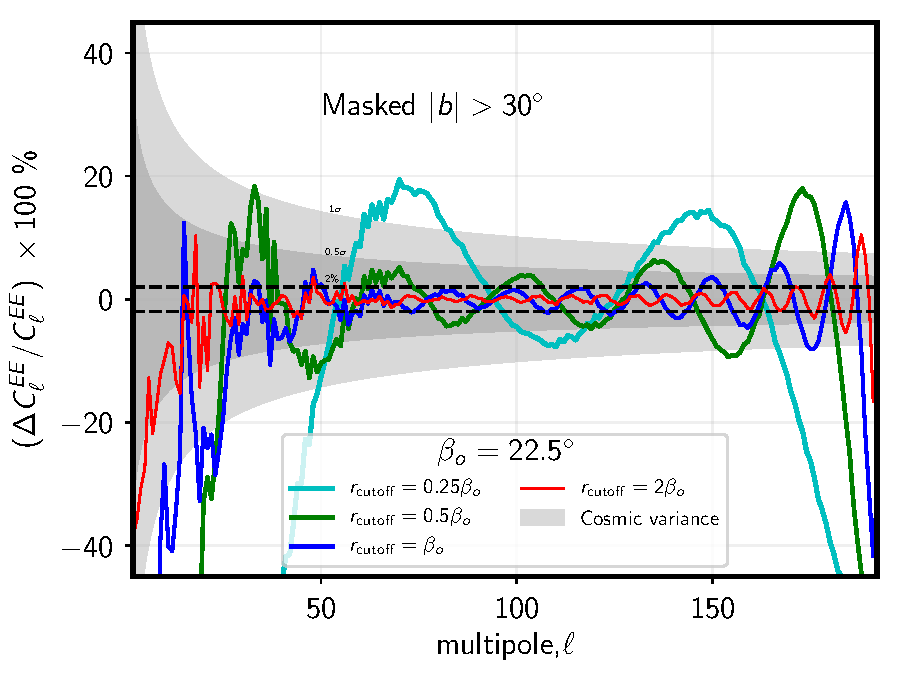
\includegraphics[width=0.49\columnwidth]{relative-percentage-err-ee-spectrum-radial-cutoff.pdf}}
\subfigure[]{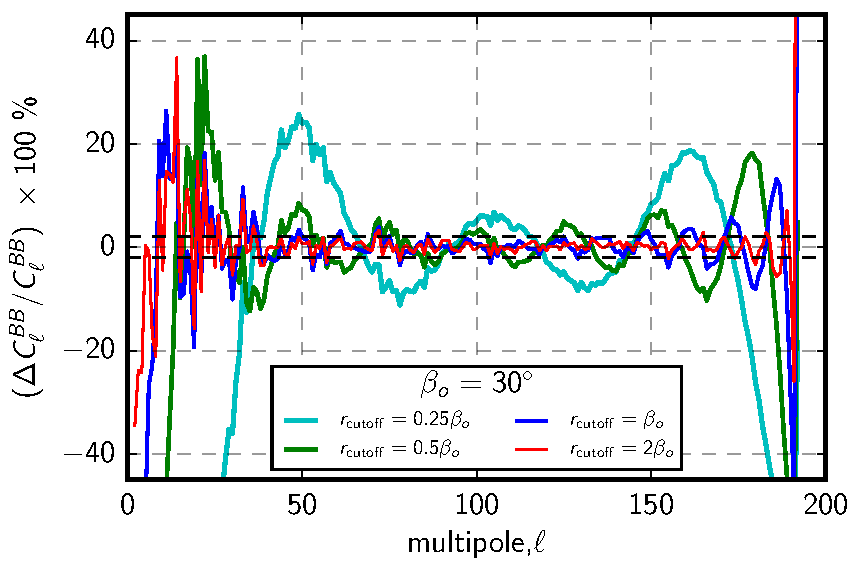
\includegraphics[width=0.49\columnwidth]{relative-percentage-err-bb-spectrum-radial-cutoff.pdf}}
\caption{}
\label{fig:eq-spectra_rad_cutoff}
\end{figure}
%
%--------------------------------------------------------
%--------------------------------------------------------
\subsection{Extracting Equ and Bqu maps}
%
\begin{figure}[!h] 
\centering
\subfigure[E-Q map Healpix]{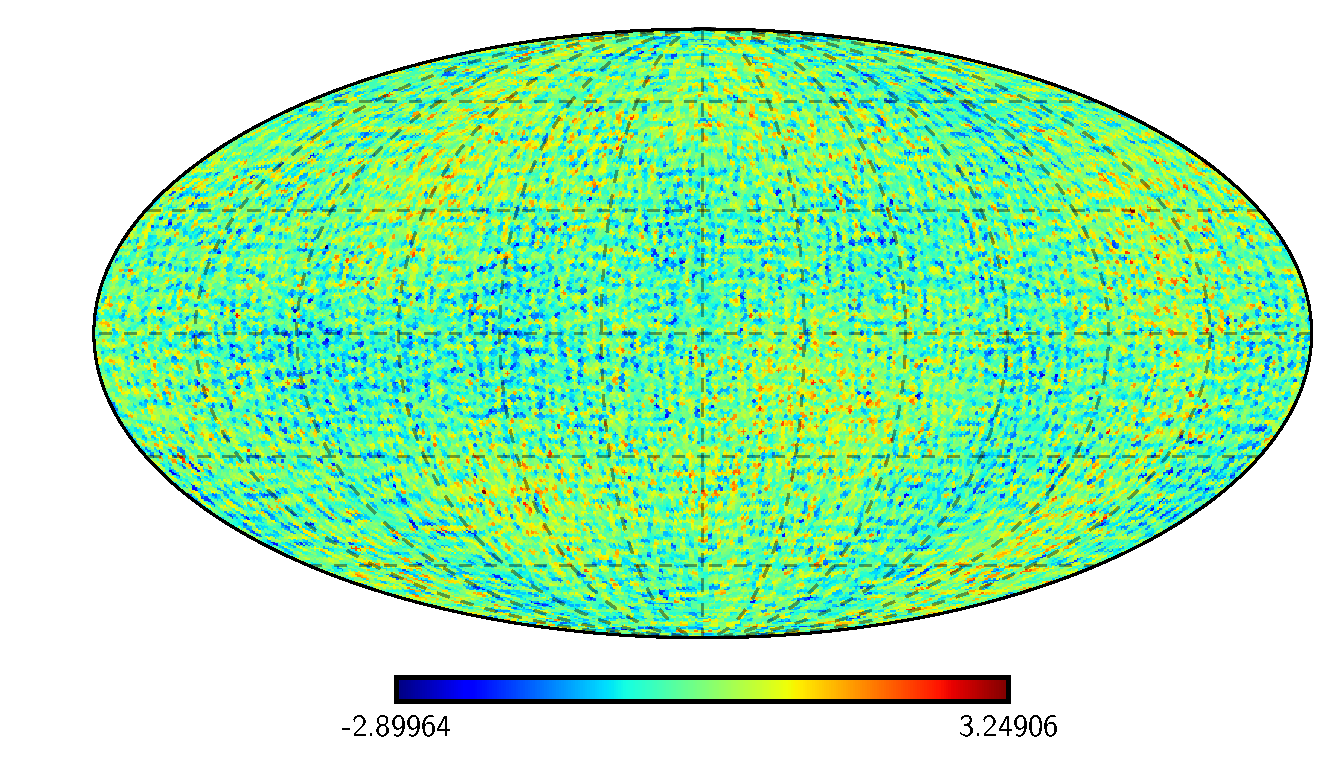
\includegraphics[width=0.31\columnwidth]{e-qmap-healpix.pdf}}
\subfigure[E-Q map local convolution]{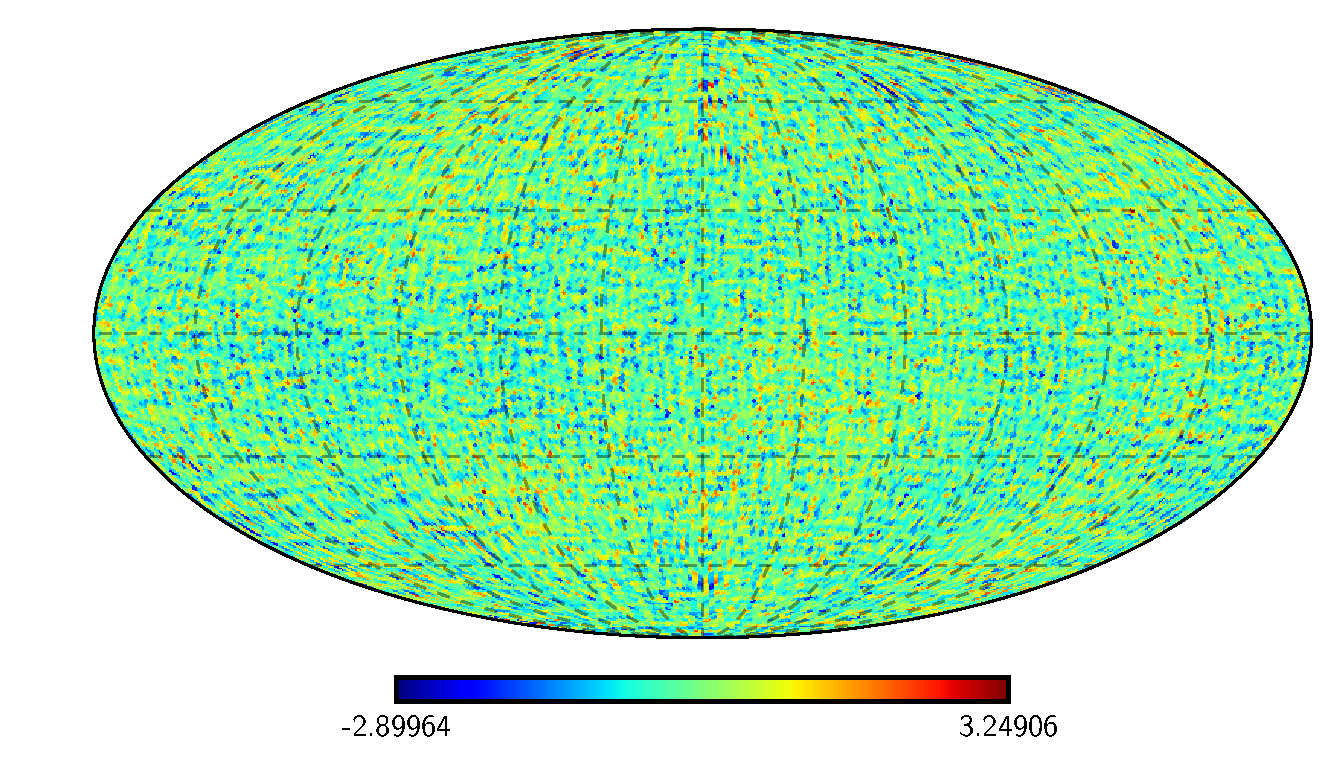
\includegraphics[width=0.31\columnwidth]{e-qmap-2beta.pdf}}
\subfigure[E-Q map difference]{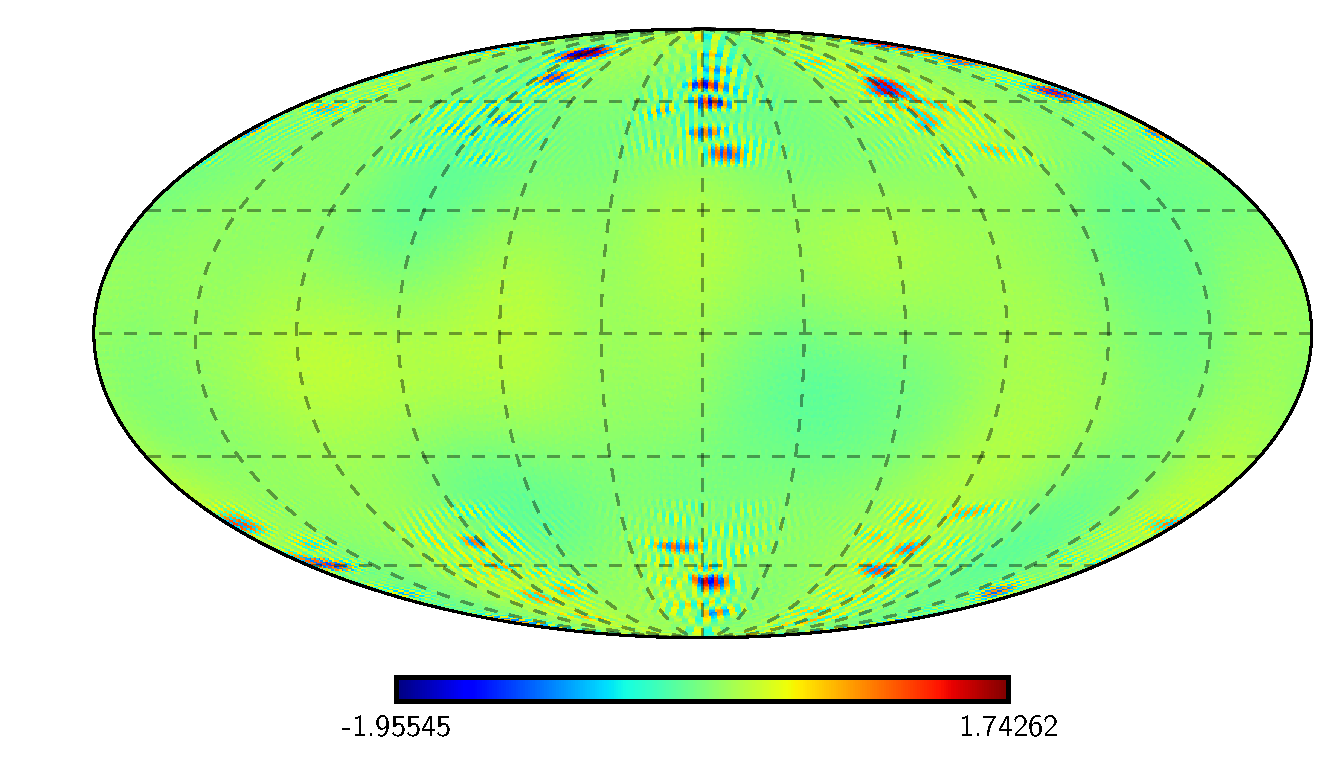
\includegraphics[width=0.31\columnwidth]{e-qmap-diff.pdf}}
\subfigure[E-U map Healpix]{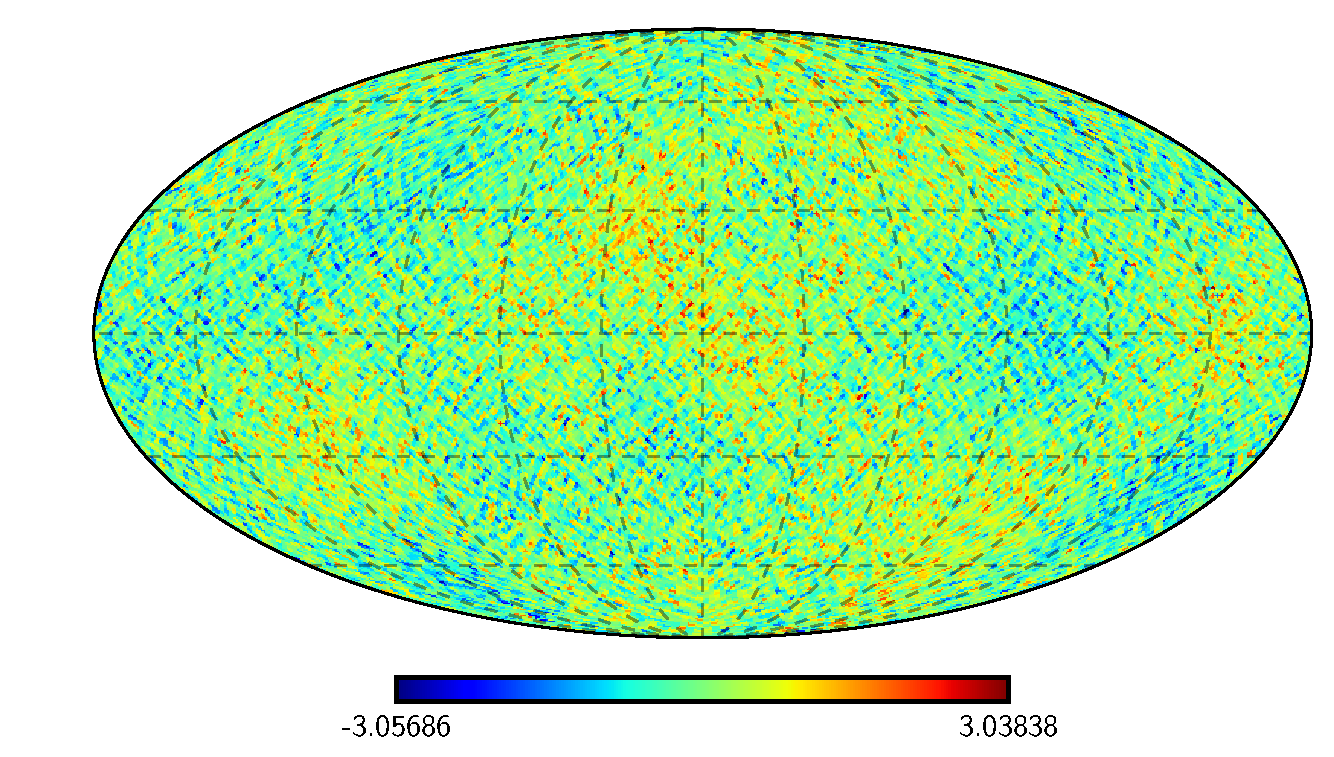
\includegraphics[width=0.31\columnwidth]{e-umap-healpix.pdf}}
\subfigure[E-U map local convolution]{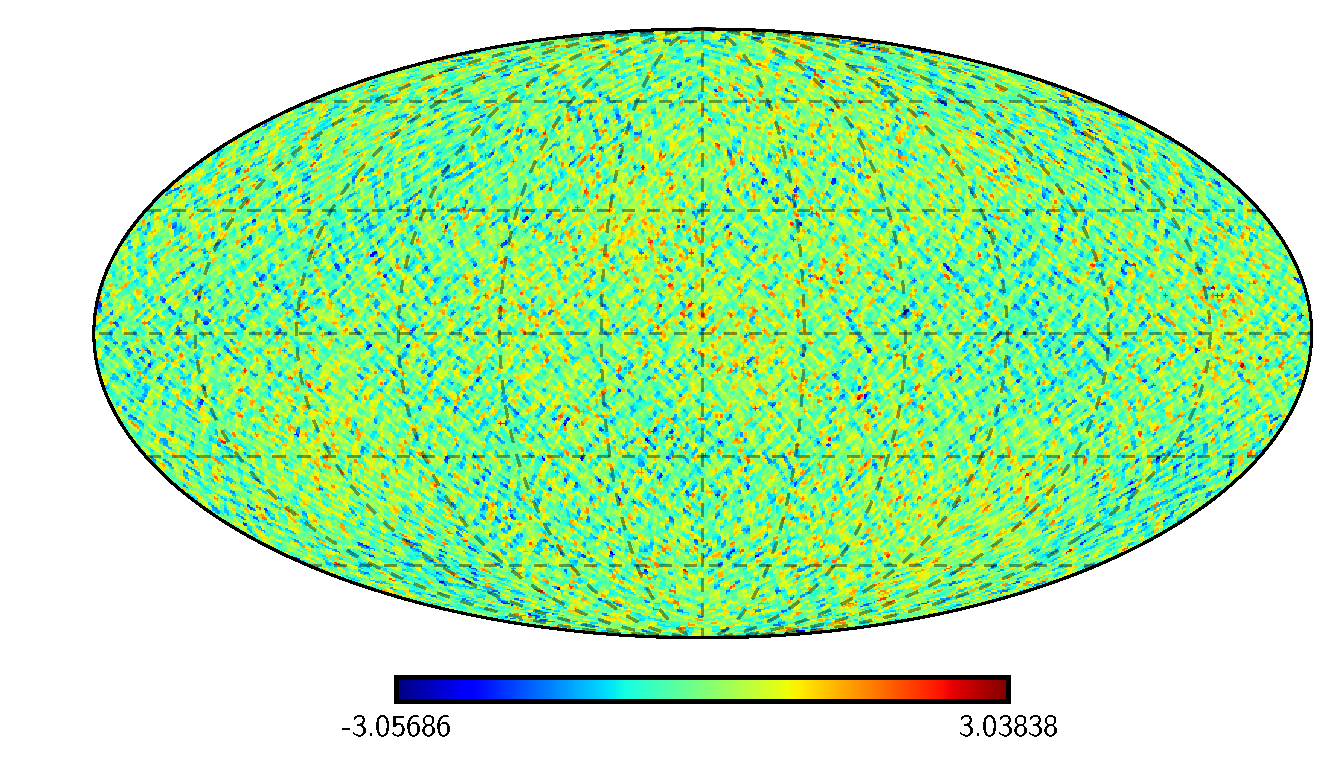
\includegraphics[width=0.31\columnwidth]{e-umap-2beta.pdf}}
\subfigure[E-U map difference]{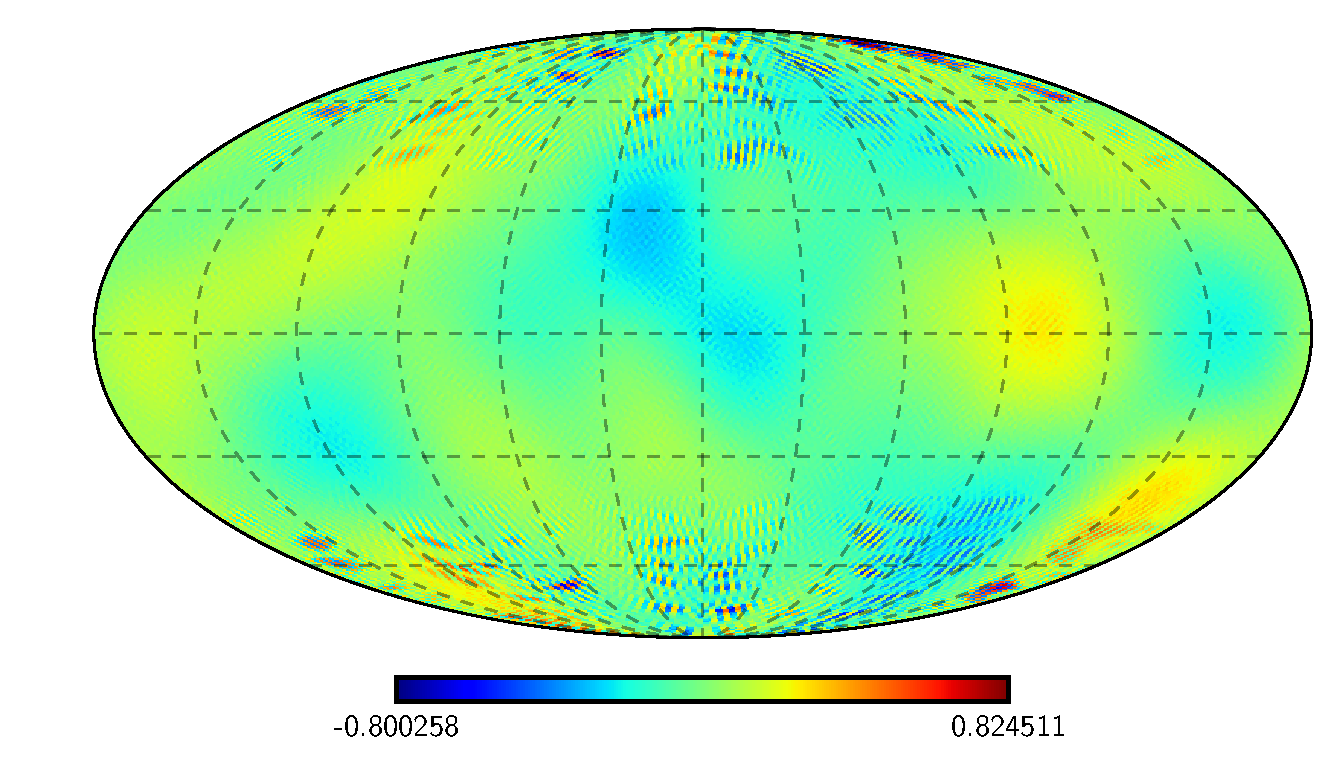
\includegraphics[width=0.31\columnwidth]{e-umap-diff.pdf}}

\subfigure[B-Q map Healpix]{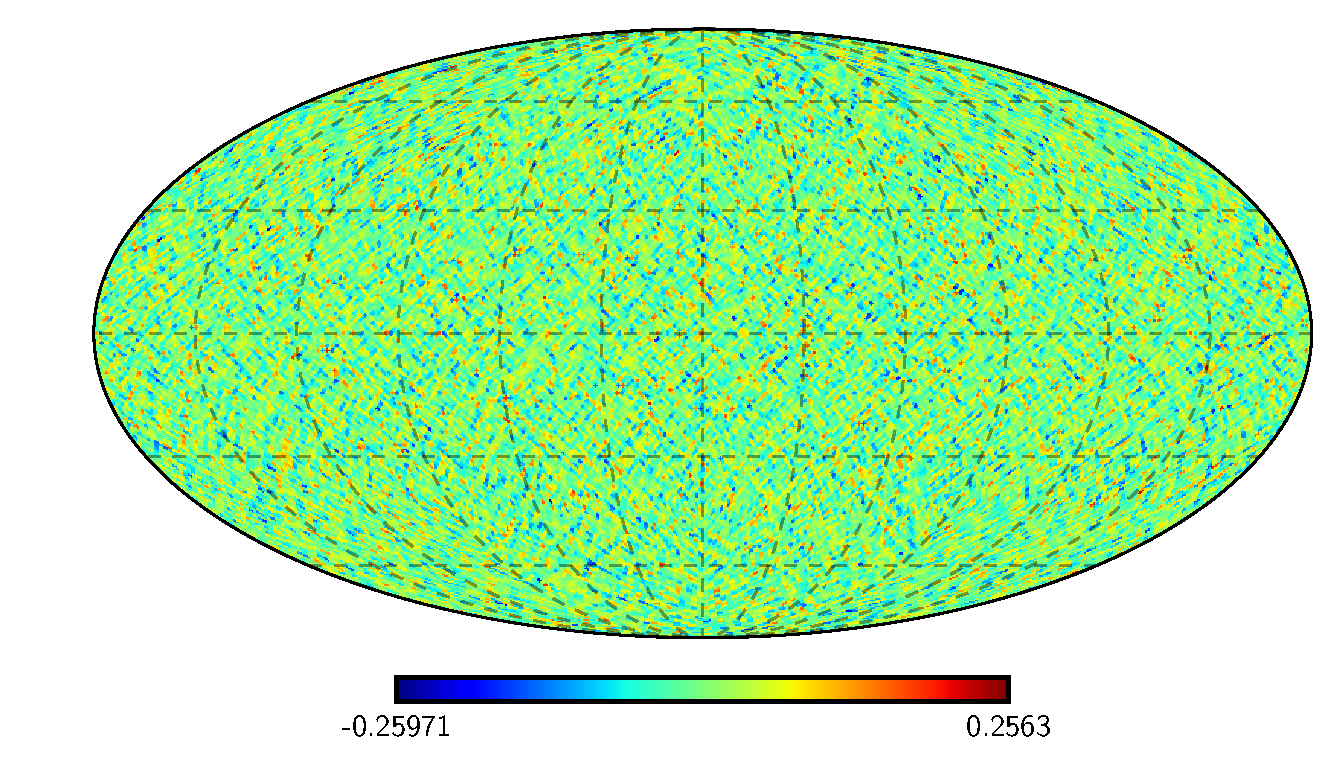
\includegraphics[width=0.31\columnwidth]{b-qmap-healpix.pdf}}
\subfigure[B-Q map local convolution]{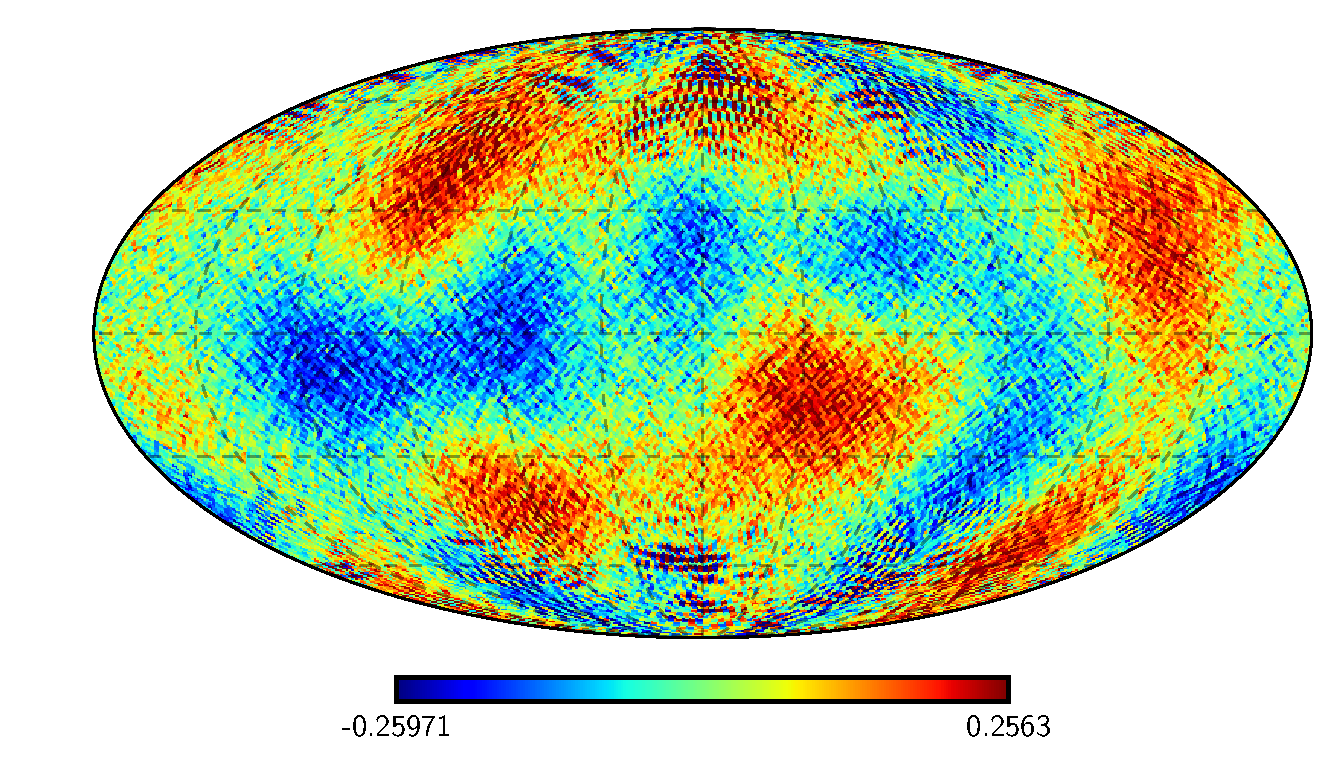
\includegraphics[width=0.31\columnwidth]{b-qmap-2beta.pdf}}
\subfigure[B-Q map difference]{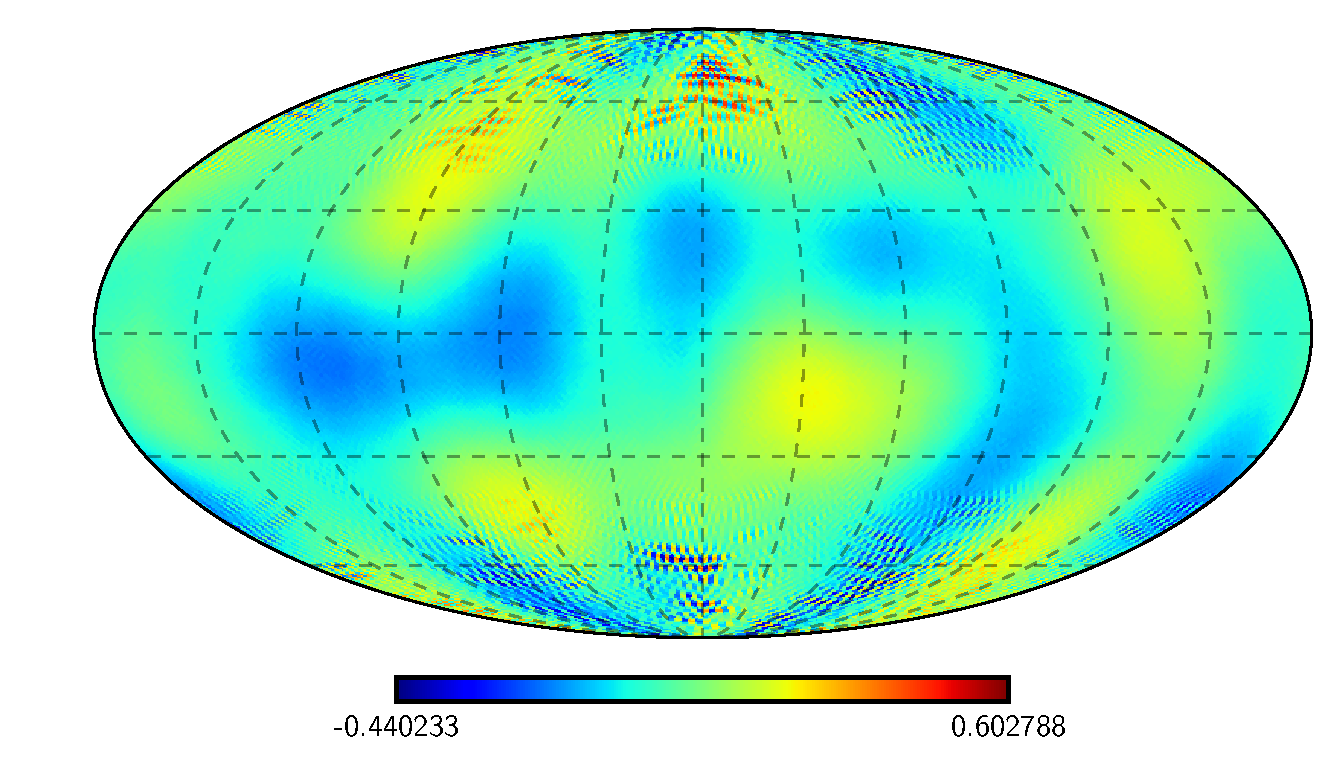
\includegraphics[width=0.31\columnwidth]{b-qmap-diff.pdf}}
\subfigure[B-U map Healpix]{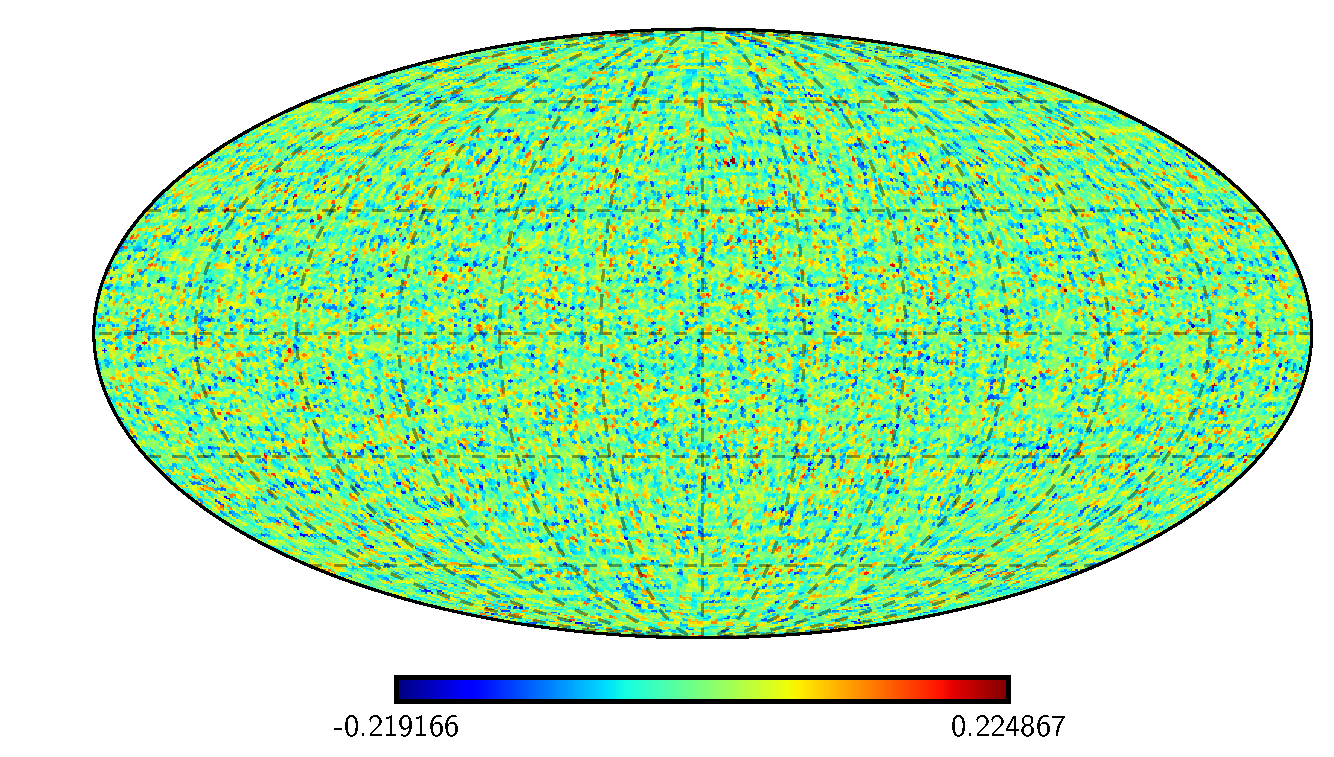
\includegraphics[width=0.31\columnwidth]{b-umap-healpix.pdf}}
\subfigure[B-U map local convolution]{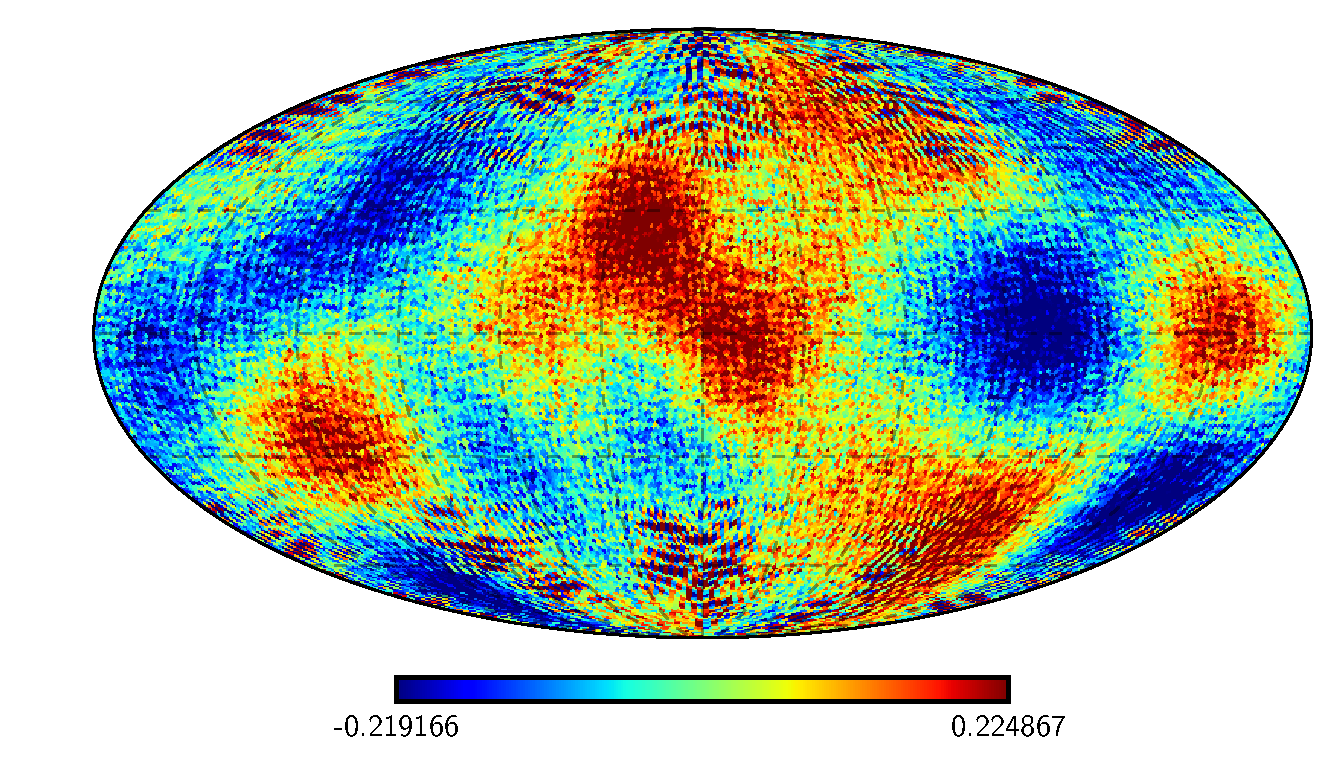
\includegraphics[width=0.31\columnwidth]{b-umap-2beta.pdf}}
\subfigure[B-U map difference]{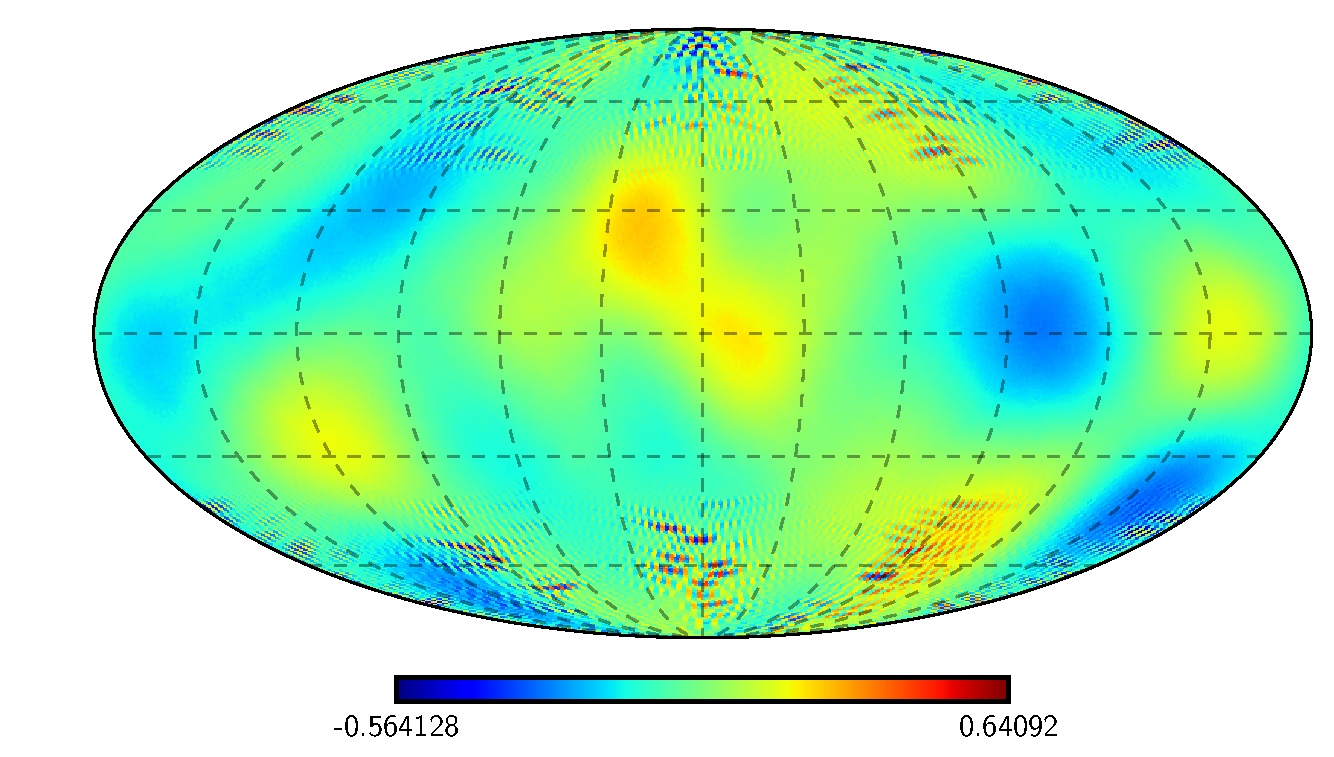
\includegraphics[width=0.31\columnwidth]{b-umap-diff.pdf}}
\caption{}
\label{fig:equ-bqu-maps-compare}
\end{figure}
%

%
\begin{figure}[!h] 
\centering
\subfigure[]{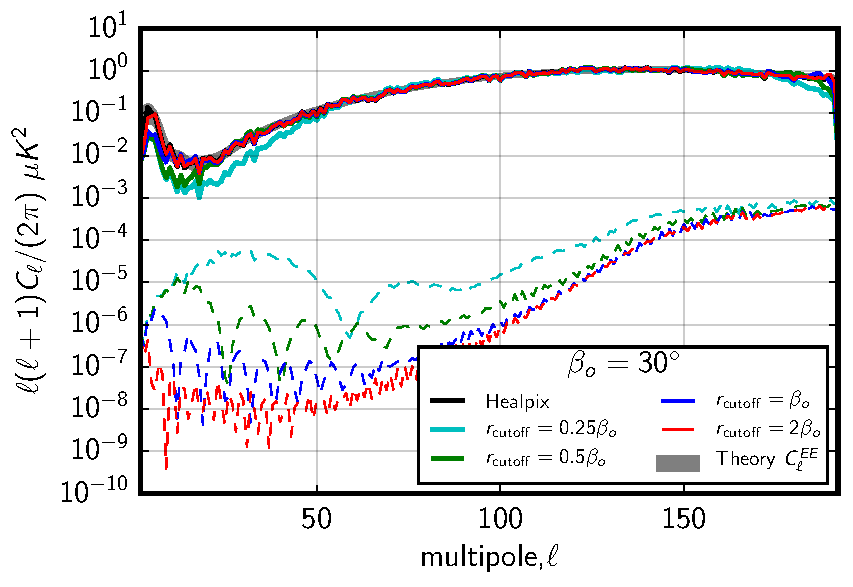
\includegraphics[width=0.49\columnwidth]{equ-spectra-radial-cutoff.pdf}}
\subfigure[]{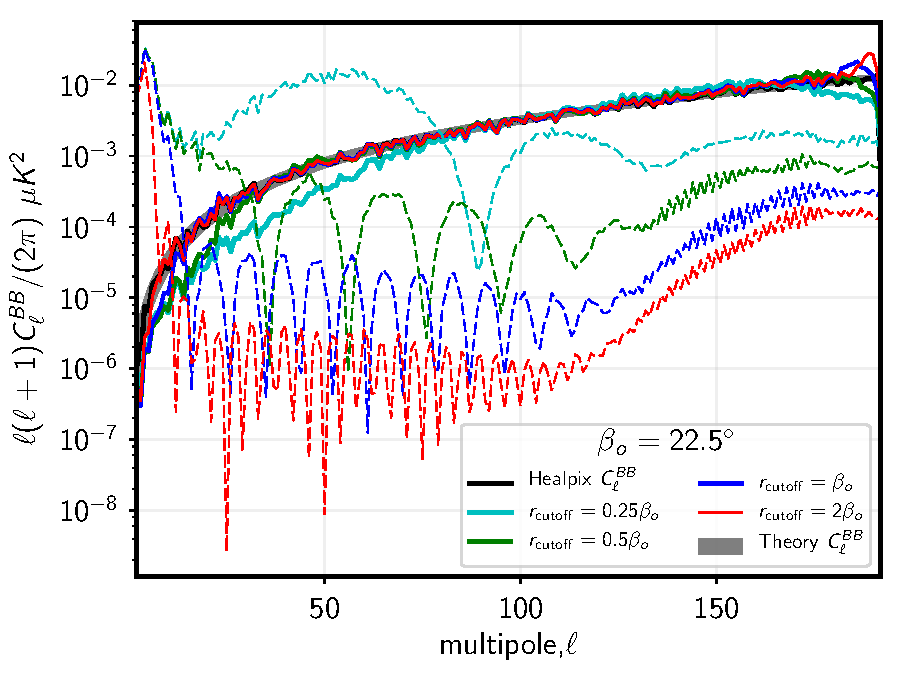
\includegraphics[width=0.49\columnwidth]{bqu-spectra-radial-cutoff.pdf}}
\subfigure[]{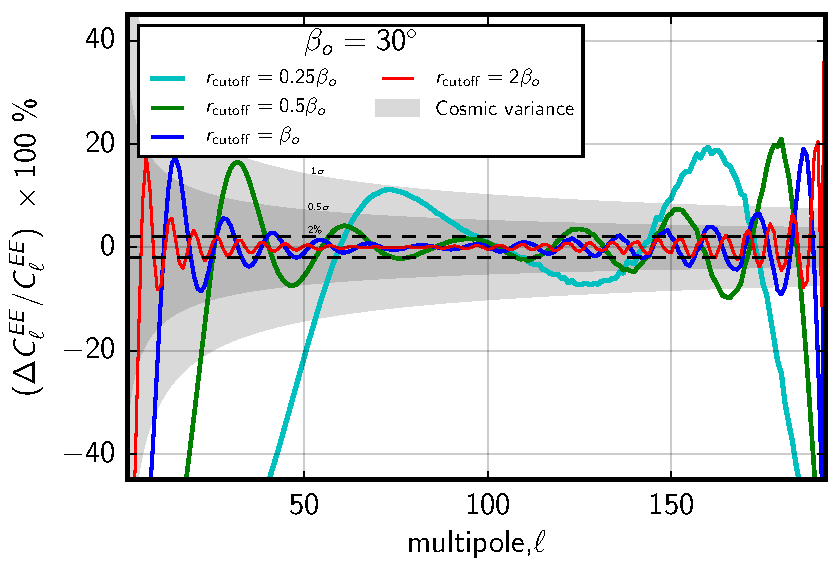
\includegraphics[width=0.49\columnwidth]{relative-percentage-err-equ-e-spectrum-radial-cutoff.pdf}}
\subfigure[]{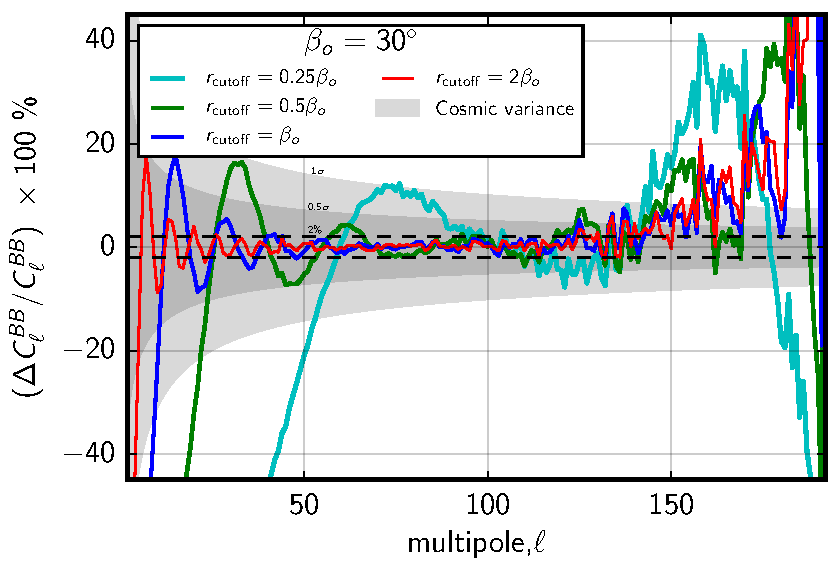
\includegraphics[width=0.49\columnwidth]{relative-percentage-err-bqu-b-spectrum-radial-cutoff.pdf}}
\caption{}
\label{fig:equ-bqu-spectra_rad_cutoff}
\end{figure}
%
%--------------------------------------------------------
%--------------------------------------------------------
\subsection{Scaling and future prospects}
%
\begin{figure}[!h] 
\centering
\subfigure[]{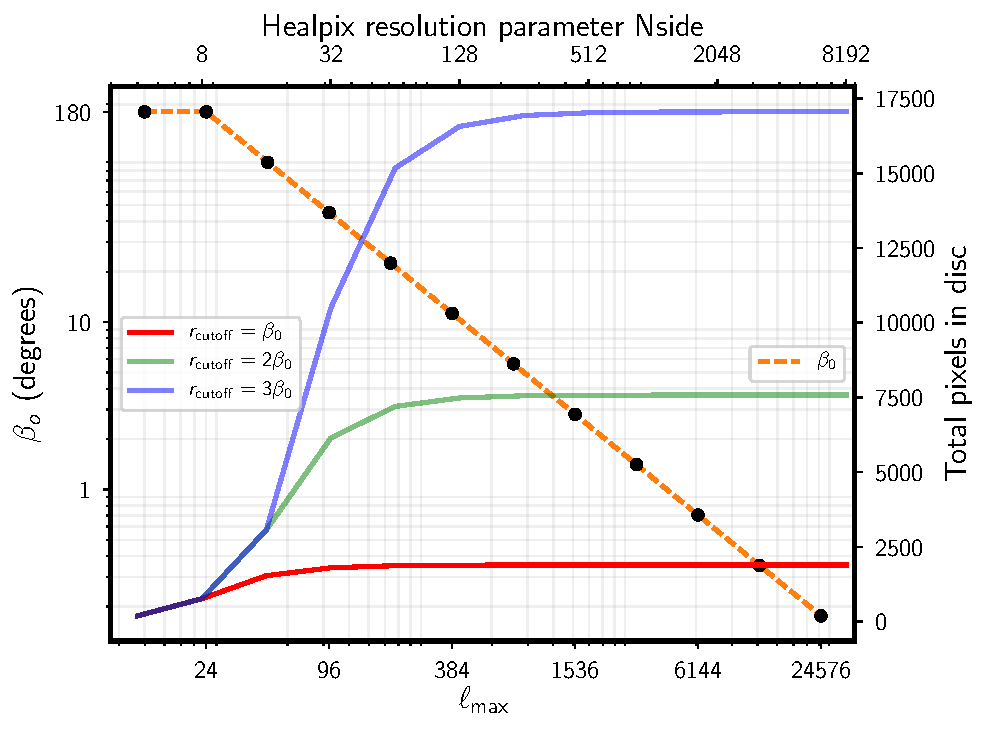
\includegraphics[width=0.8\columnwidth]{number_of_disc_pixels.pdf}}
\caption{The red dashed curve depicts the how $\beta_o$ changes as a function of the Healpix resolution parameter Nside assuming that the maximum multipole accessible in the map is given by $\ell_{\rm max} = 3 * Nside$. The blue solid curve depicts the number of surrounding pixel that will need to be accessed to carry out the convolution on Stokes Q \& U maps to infer the value of the scalar fields E \& B at the central pixel.}
\label{fig:disc_rad_healpix_numpix}
\end{figure}
%
%--------------------------------------------------------
%--------------------------------------------------------
